\documentclass[xetex,mathserif,serif]{beamer}

\setbeamertemplate{caption}[numbered]
% Hyperlinks.
\usepackage{hyperref}

% Language settings.
\usepackage{polyglossia}
\setdefaultlanguage[babelshorthands=true]{russian}

% Setting outer theme.
\useoutertheme{infolines}

% Setting font.
\usepackage{fontspec}
\setmainfont{FreeSans}
\newfontfamily{\russianfonttt}{FreeSans}

% Code highlighting.
\usepackage[outputdir=build]{minted}
\usepackage{xcolor}

% Images.
\usepackage{graphicx}
\usepackage{animate}
\usepackage{subfig}


\usepackage{mathtools}

\title[СПбГУ]{Построение гибридной рекомендательной
системы новостей с применением методов
оптимизации}
\author[Смирнов Александр 17.Б07-мм]{Смирнов Александр 17.Б07-мм}
\institute[]{Научный руководитель: к.ф.-м.н., доц. Михайлова Елена Георгиевна \\
             Рецензент: руководитель отдела инженерии ООО ``АЙ ТИ Сервис'', Осипов Евгений Валерьевич}
% \author[Alexander Smirnov]{Alexander Smirnov\\ \footnotesize supervisor: Elena Mikhailova}

\begin{document}


\frame{\titlepage}

% \section{Introduction}

% \subsection{Approaches}

\begin{frame}
	\frametitle{Введение}

	\begin{itemize}
		\item Приложение ЯRUS:
		      \begin{itemize}
			      \item Агрегатор новостей;
			      \item Социальная сеть;
		      \end{itemize}
		\item Огромный объём информации:
		      \begin{itemize}
			      \item Необходима персонализация.
		      \end{itemize}
	\end{itemize}

\end{frame}



\begin{frame}
	\frametitle{Постановка задачи}

	\begin{itemize}
		\item Цель:
            \begin{itemize}
                \item Реализация рекомендательной системы новостей в приложении ЯRUS;
            \end{itemize}

		\item Задачи:
            \begin{itemize}
                \item Исследование предметной области;
                \item Анализ проблем существующих подходов;
                \item Реализация подходов;
                \item Совмещение подходов в единую систему;
                \item Анализ качества работы рекомендательной системы;
                \item Оценка влияния решения на ключевые показатели эффективности.
            \end{itemize}
	\end{itemize}
\end{frame}


\begin{frame}
	\frametitle{Подходы}

	\begin{itemize}
		\item Коллаборативная фильтрация;
		\item Фильтрация на основе содержимого;
		\item Фильтрация на основе популярности.
	\end{itemize}
\end{frame}

\begin{frame}
	\frametitle{Коллаборативная фильтрация}

	\begin{itemize}
		\item Рекомендации в зависимости от истории похожих пользователей;
		\item Проблемы:
		      \begin{itemize}
			      \item Холодный старт;
			      \item Вычислительные сложности;
                  \item Отзывчивость системы на действия пользователей;
			      \item Разреженность данных.
		      \end{itemize}
	\end{itemize}
\end{frame}

\begin{frame}
	\frametitle{Фильтрация на основе содержимого}

	\begin{itemize}
		\item Рекомендации в зависимости от истории взаимодействия пользователя;
		\item Проблемы:
		      \begin{itemize}
			      \item Холодный старт;
			      \item Векторизация рекомендуемого предмета;
			      \item Однообразность содержимого.
		      \end{itemize}
	\end{itemize}
\end{frame}

\begin{frame}
	\frametitle{Фильтрация на основе популярности}

	\begin{itemize}
		\item Рекомендуемые самые ``трендовые'' новости;
		\item Проблемы:
		      \begin{itemize}
			      \item Отсутствие персонализации.
		      \end{itemize}
	\end{itemize}
\end{frame}



\begin{frame}
	\frametitle{Описание подхода}

    \begin{figure}[h]
        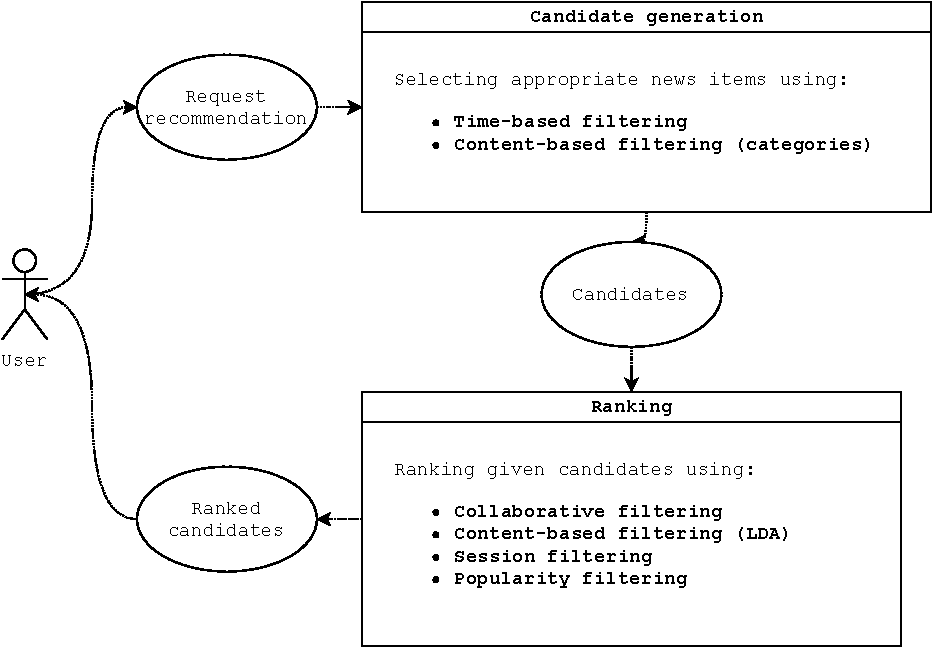
\includegraphics[width=0.7\textwidth]{./images/architechture.pdf}
        \caption{Обзор подхода}
        \label{fig:arch}
        \centering
    \end{figure}

\end{frame}

\begin{frame}
    \frametitle{Описание подхода (продолжение)}

	\begin{itemize}
        \item Отбор кандидатов:
            \begin{itemize}
                \item Штраф за устаревание новости;
                \item Грубая фильтрация по категориям;
            \end{itemize}
        \item Ранжирование:
            \begin{itemize}
                \item Коллаборативная фильтрация;
                \item Фильтрация на основе содержимого;
                \item Фильтрация на основе текущей сессии;
                \item Фильтрация на основе популярности.
            \end{itemize}
	\end{itemize}
\end{frame}

\begin{frame}
    \frametitle{Описание подхода (продолжение)}

	\begin{itemize}
        \item Решённые проблемы:
            \begin{itemize}
			    \item Холодный старт;
			    \item Вычислительные сложности;
                \item Отзывчивость системы на действия пользователей;
			    \item Векторизация рекомендуемого предмета;
			    \item Однообразность содержимого;
			    \item Отсутствие персонализации.
            \end{itemize}
	\end{itemize}
\end{frame}



\begin{frame}
    \frametitle{Фильтрация на основе содержимого}

	\begin{itemize}
		\item 
	\end{itemize}
\end{frame}

\begin{frame}
    \frametitle{Коллаборативная фильтрация}

	\begin{itemize}
		\item 
	\end{itemize}
\end{frame}

\begin{frame}
    \frametitle{Оценка качества (offline)}

	\begin{itemize}
		\item MAP@20
		\item NDCG
		\item 
	\end{itemize}
\end{frame}


\begin{frame}
	\frametitle{Оценка качества (online)}

	\begin{itemize}
		\item A/B тестирование:
            \begin{itemize}
                \item Время нахождения на вкладке ``новости'' за одну сессию;
                \item Вовлечённость:
                    \begin{itemize}
                        \item Количество эмоций;
                        \item Количество комментариев.
                    \end{itemize}
            \end{itemize}
		\item 
		\item 
	\end{itemize}
\end{frame}





\begin{frame}
	\frametitle{Внедрение}

	\begin{itemize}
		\item Микросервисная архитектура:
            \begin{itemize}
                \item Алгоритмы рекомендаций;
                \item Алгоритмы подготовки и обработки данных;
            \end{itemize}
		\item python, flask: разработка;
		\item docker: упаковка решений;
		\item k8s: оркестрация;
		\item gitlab: версионирование; 
		\item gitlab CI: непрерывная интеграция.
	\end{itemize}
\end{frame}



\begin{frame}
	\frametitle{Апробация}

    \begin{figure}[h]
        
\includegraphics[width=0.3\textwidth]{./images/screenshot.png}
        \caption{Персонализированная рекомендательная лента}
        \label{fig:feed}
        \centering
    \end{figure}

\end{frame}


\begin{frame}
	\frametitle{Результаты}
	\begin{itemize}
		\item Проведён обзор существующих решений;
		\item Собрано уникальное решение;
		\item Оценено качество предложенного решения;
		\item Решение реализовано и внедрено в экосистему приложения ЯRUS;
		\item Увеличено время нахождения пользователей в приложении и повышена вовлёченность.
	\end{itemize}
\end{frame}


\begin{frame}
	\frametitle{Акт о внедрении}

    \begin{figure}[h]
        
\includegraphics[width=0.45\textwidth]{./images/akt.jpg}
        \caption{Акт о внедрении}
        \label{fig:akt}
        \centering
    \end{figure}

\end{frame}

\begin{frame}
	\frametitle{Заключение}


    \begin{itemize}
        \item Спасибо за внимание!
        \item Задавайте вопросы.
    \end{itemize}

    \begin{itemize}
        \item Ссылки:
            \begin{itemize}
                \item \href{https://yarus.ru/}{yarus.ru}
                \item \href{https://t.me/furiousteabag}{@furiousteabag}
            \end{itemize}
    \end{itemize}


\end{frame}

\end{document}
